\section*{Exercício 7}
\label{ex:7}

Os dados utilizadas na simulação está na tabela \ref{tab:ex7}. A imagem \ref{fig:dcIntrocomplete} apresenta o resultado das quatro estratégias utilizadas para controlar a velocidade de um motor DC. Todas implementam um controlador PID com discretização para trás para partes I e D. Entretanto, o sinal laranja apresenta a estratégia de anti-windup a qual desativa a ação integradora durante a saturação, o sinal amarelo apresenta a mesma estratégia com um filtro passa-baixas associado ao termo derivativo e, por fim, o sinal em púrpura utiliza a diferença entre a ação anterior de controle e a atual para mitigar a ação de controle durante a saturação.

\begin{table}[H]
    \centering
    \begin{tabular}{|l|c|c|c|}
    \hline
    Descrição & Símbolo & Unidade & Valor \\ \hline
    Resistência do estator & R & $\Omega$ & 1 \\
    Indutância do estator & L & H & 0.01 \\
    Momento de inércia & J & kg $m^2$  & 1 \\
    Coeficiente de atrito viscoso & b & $N \frac{rad}{s}$ & 0.01 \\
    Fator transformação eletromagnética & K & NmA & 1 \\\hline
    \end{tabular}
    \caption{Parâmetros da planta}
    \label{tab:ex7}
\end{table}

\begin{table}[H]
    \centering
    \begin{tabular}{|l|c|c|c|}
    \hline
    Descrição & Símbolo & Unidade & Valor \\ \hline
    Ganho proporcional & $K_p$ & $N \frac{rad}{s}$ & 18 \\
    Constante de tempo integrativo & $T_i$ & s & 0.42 \\
    Constante de tempo derivativo & $T_d$ & s  & 0.05 \\
    Período de amostragem & $T_s$ & s & 0.01 \\\hline
    \end{tabular}
    \caption{Parâmetros do controlador}
    \label{tab:ex7}
\end{table}

Os sinais apresentam uma semelhança qualitativa, entretanto, a ação de controle 

Deseja-se avaliar a performance dos controladores com respeito à saturação e 

\begin{figure}[H]
    \center
    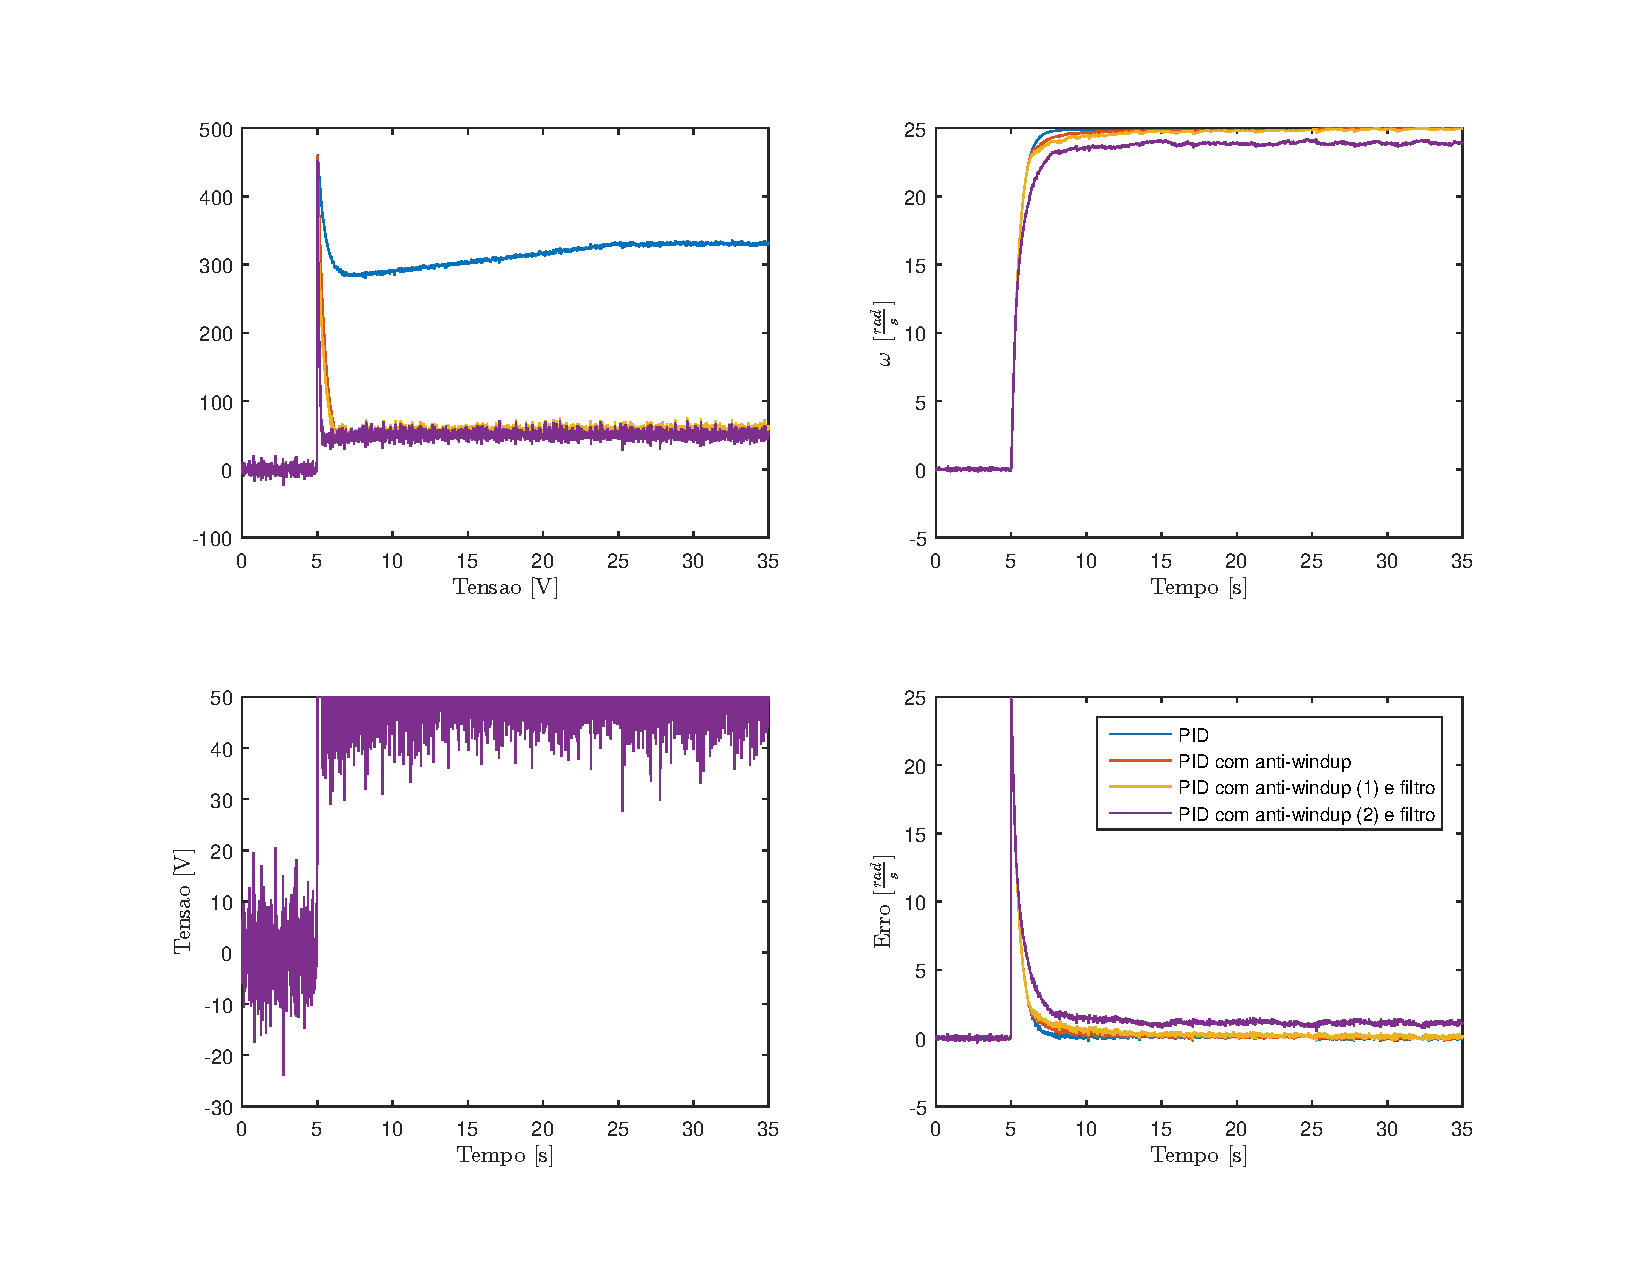
\includegraphics[width=1.2\textwidth, trim=4cm 2cm 1cm 1cm]{ex7.pdf}
    \caption{Principais sinais de controle do diagrama} \label{fig:dcIntrocomplete}
\end{figure}

\begin{figure}[H]
    \center
    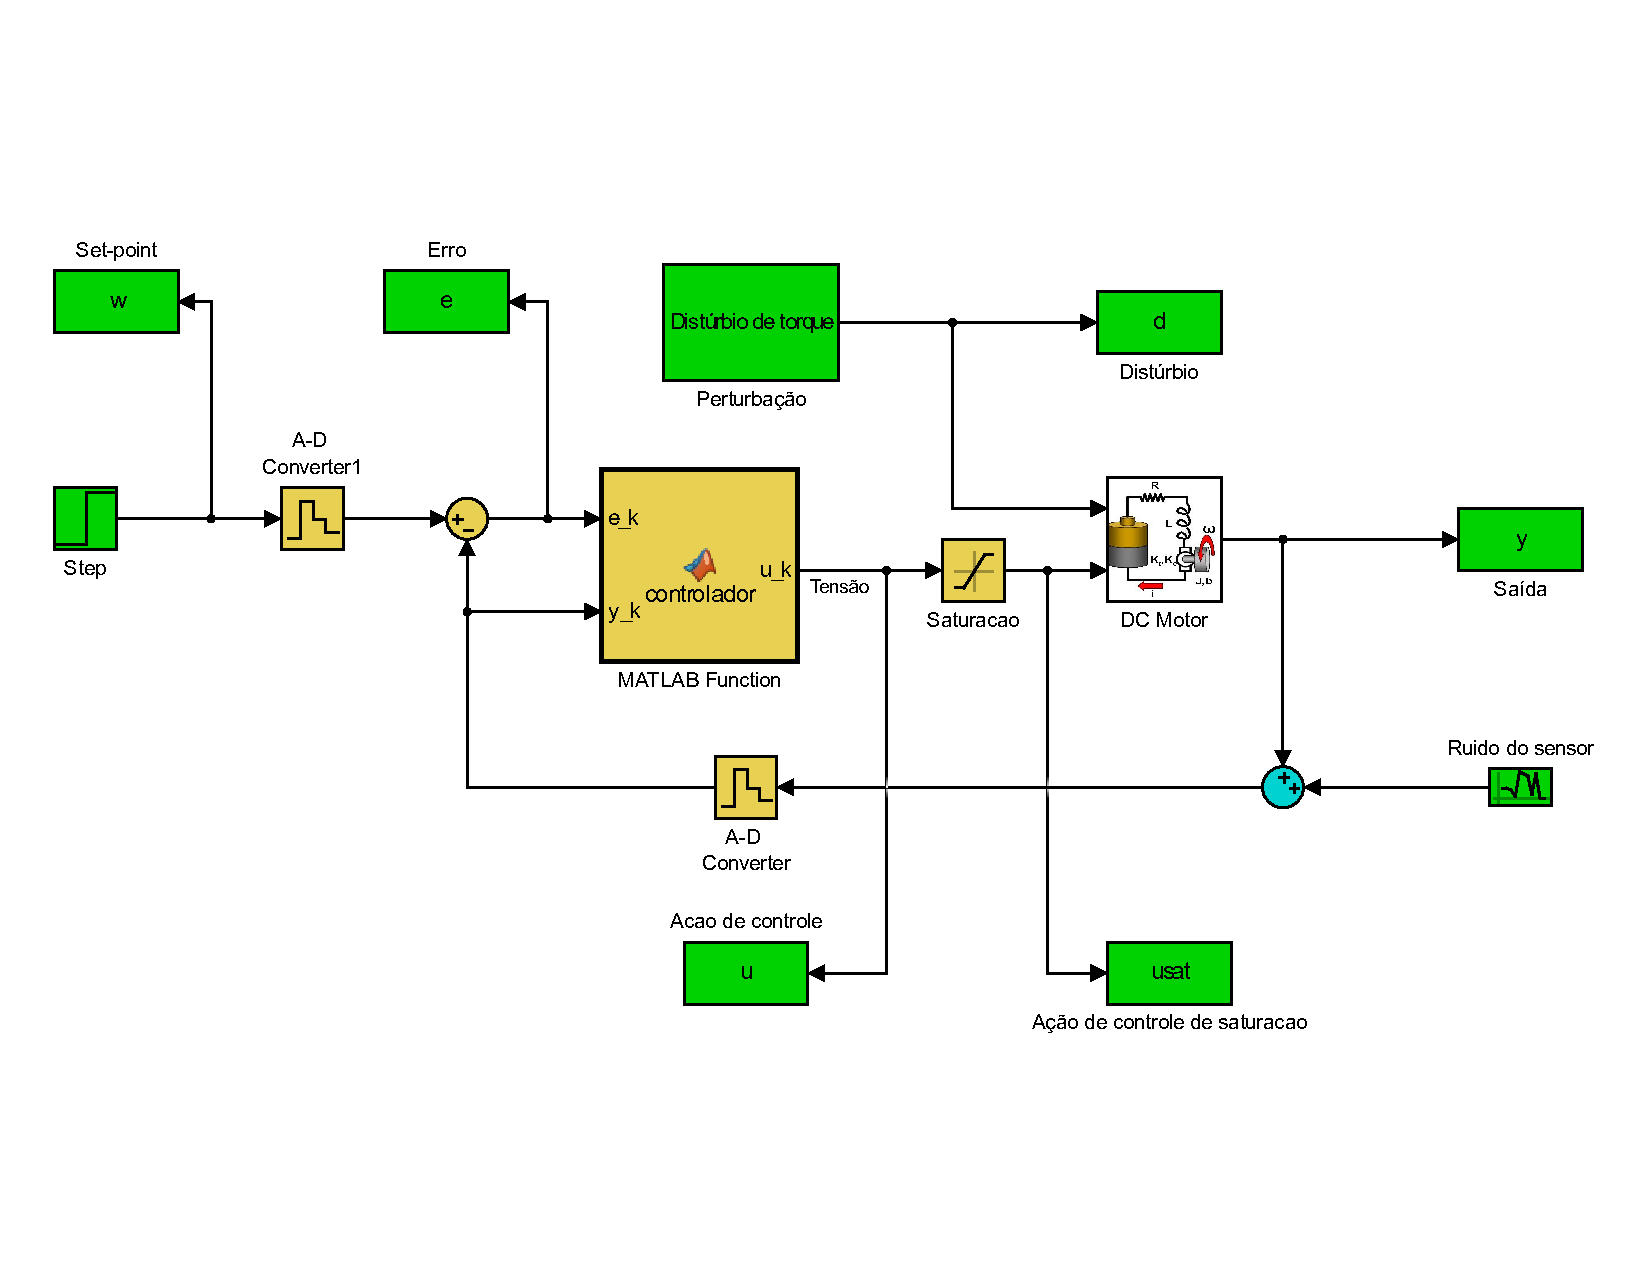
\includegraphics[width=0.8\textwidth, trim=3.5cm 3.5cm 2cm 2cm]{dcIntrocomplete.pdf}
    \caption{Diagrama de blocos utilizado para exercício 7}
    \label{fig:ex7}
\end{figure}

